\bilingualchapter{Volatility targeting}{波动率目标设定}

\begin{englishblock} DO YOU REMEMBER SERGEI, DISPENSER OF OPAQUE TRADING advice in chapter seven? He told me that there were three issues to consider when deciding how big a position we should have. The first thing to consider was how much we liked the trade. You've dealt with that by creating a single forecast for each instrument you're trading -- either a discretionary forecast for semi-automated traders, a constant forecast for asset allocating investors, or a combined forecast for staunch systems traders. Now we're ready to return to Sergei's second question, "How much can you afford to lose?"96 \end{englishblock}

\begin{chineseblock}你还记得第七章里那位以晦涩交易建议著称的 Sergei 吗？他说过，当我们决定应该持有多大仓位时，需要考虑三个问题。第一个问题是，你到底有多看好这笔交易。这个问题你已经解决了：你已经为每个交易品种生成了一个单一预测值--- 对半自动交易者来说，这是主观预测；对资产配置型投资者来说，这是恒定预测；对坚定的系统化交易者来说，则是合成预测。现在，我们已经准备好回到 Sergei 的第二个问题了：“你最多能承受多大亏损？”96 \end{chineseblock}

\bilingualsection{Chapter overview}{本章概览}

\begin{bilingualtableblock} \begin{tabularx}{\textwidth}{@{} L{0.30\textwidth} Y@{}}\textbf{The importance of risk targeting} & Why getting your appetite for risk right is so important and the key issues involved. \\

\textbf{风险目标设定的重要性} & 为什么把风险偏好设定正确如此重要，以及其中涉及的关键问题。 \\
\textbf{Setting your volatility target} & The measure of how much risk you’re prepared to take and how to calculate it. \\
\textbf{设定你的波动率目标} & 你愿意承担多少风险的度量方式，以及如何计算它。 \\
\textbf{Rolling up profits and losses} & How your volatility target should be adjusted when you lose or make money. \\
\textbf{将盈亏滚动纳入资本} & 当你亏钱或赚钱时，波动率目标应当如何随之调整。 \\
\textbf{What percentage of capital per trade} & Relating the volatility targeting concept to traditional money management where you limit bets to a specific percentage of capital. \\
\textbf{每笔交易占用资本的百分比} & 把波动率目标设定的概念与传统资金管理联系起来； 传统资金管理会把每笔下注限制在资本的一定百分比之内。 \\
\end{tabularx}
\end{bilingualtableblock}

\bilingualsection{The importance of risk targeting}{风险目标设定的重要性}

\begin{englishblock} Deciding your overall trading risk is the most important decision you will have to make when designing your trading system. Nearly all amateur traders lose money and most do so because their positions are too large compared to their account size.\footnote{The other reason is that they trade too much, which is covered in chapter twelve, ‘Speed and Size'. \par 另一个原因是他们交易得过于频繁，这一点会在第十二章“速度与规模”中讨论。} Suffering painful losses is the main reason why both amateurs and professionals meddle with trading systems rather than letting them run unimpeded. Making this decision correctly involves understanding two things. Firstly you must understand your system, in particular its likely performance and whether it's likely to have positive or negative skew. You must avoid overconfidence, as I discussed in chapter one. You should not extrapolate over-fitted back-test results to create high expectations of return. Are you sure your strategy can generate a Sharpe ratio of 2.0 after costs? Are you really, really sure? Next you must understand yourself, in a complete and honest way. Can you face the possibility of regularly losing 5\%, 10\% or 20\% of your own capital in a day? These points also apply to those paid to manage other people's money. Additionally professionals need to understand their clients' tolerance for losing money. If investors aren't truly comfortable with the risks being taken then you will see them redeeming in droves when large losses occur. \end{englishblock}

\begin{chineseblock}在设计交易系统时，决定整体交易风险，是你必须做出的最重要决定。几乎所有业余交易者都会亏钱，而其中大多数之所以亏钱，是因为他们的仓位相对于账户规模来说太大了。痛苦的亏损，是业余人士和专业人士都会去干预交易系统、而不是让系统顺畅运行的主要原因。要想把这个决定做对，就必须理解两件事。第一，你必须理解自己的系统，尤其是它可能的表现，以及它更可能呈现正偏度还是负偏度。正如我在第一章中讨论过的，你必须避免过度自信。你不应当拿那些过拟合的回测结果去外推，进而形成过高的收益预期。你真的确定自己的策略在扣除成本后能够实现 2.0 的夏普比率吗？你真的、真的确定吗？其次，你还必须以完全而诚实的方式理解你自己。你能否面对自己的资本在一天之内规律性地亏掉 5\%、10\% 或 20\% 的可能性？这些问题同样适用于那些受雇管理他人资金的人。此外，专业人士还必须理解客户对亏损的承受能力。如果投资者并不真正接受你正在承担的风险，那么一旦出现大额亏损，你就会看到他们成群结队地赎回资金。\end{chineseblock}

\bilingualsection{Setting a volatility target}{设定波动率目标}

\begin{englishblock} Imaginary conversation between a financial advisor and myself: Financial ‘expert': "How much risk do you want to take?" \end{englishblock}

\begin{chineseblock}下面是一段我和某位理财顾问之间的虚构对话：金融“专家”：“你想承担多大的风险？”\end{chineseblock}

\bilingualsubsection{Me: "What do you mean by risk?"}{我：“你说的风险是什么意思？”}

\begin{englishblock} Financial ‘expert': "Er... well how would you define your tolerance for losing money?" Me: "Well it could be how much I'm prepared to lose next year. Or tomorrow. Or next week. Are you talking about the absolute maximum loss I can cope with, or the average, or the worst loss I'd expect 95 days out of 100 (the so called ‘Value at Risk')? Which question would you like me to answer?" Financial ‘expert': "Hold on. I need to speak to my supervisor..." Joking aside, how do we answer this deceptively simple question? To keep things simple I use a single figure to measure appetite for risk -- an expected standard deviation, which I call the volatility target. You can measure this as a percentage, or in cash terms, and over different time periods. So for example the daily cash volatility target is the average expected standard deviation of the daily portfolio returns. As it's a cash value you need to specify the currency that your account or fund is denominated in. When I first discussed risk on page 39 I talked about predictable and unpredictable risks. Your volatility target is the long-term average of expected, predictable, risk. The exact predictable risk you have on any given day will depend on the strength of your forecasts, and on the current expected correlation of asset prices. You'll also face unpredictable risks if your forecast of volatility or correlations is wrong. In any case the actual amount you lose or gain on any given day will be random, since even a perfect estimation of risk only tells you what your average gains and losses will be. I find it's easier to look at an annualised cash volatility target, which will be the annualised expected daily standard deviation of returns. As before you annualise by multiplying by the square root of time; given there are around 256 trading days in a year this will be \end{englishblock}

\begin{chineseblock}金融“专家”：“呃……那你会怎么定义自己对亏钱的容忍度？”我：“那得看你问的是哪一种啊。可能是我明年最多愿意亏多少，也可能是明天，或者下周。你问的是我能承受的绝对最大亏损？还是平均亏损？还是 100 天里有 95 天不会超过的最坏亏损（也就是所谓的 ‘Value at Risk’，风险价值）？你希望我回答的是哪一个问题？”金融“专家”：“等一下，我得去问下主管……”玩笑归玩笑，我们到底该如何回答这个看似简单、实则复杂的问题？为了保持简单，我用一个单一数字来衡量风险偏好--- 一个预期标准差，我把它称为波动率目标（volatility target）。你可以用百分比来度量它，也可以用现金金额来度量它，而且还可以在不同时间尺度上表达它。例如，日现金波动率目标就是投资组合日收益的平均预期标准差。由于这是现金值，你还需要明确账户或基金使用的是哪一种计价货币。当我第一次在第 39 页讨论风险时，我提到了可预测风险与不可预测风险。你的波动率目标，其实就是长期平均意义下的、预期的、可预测风险。而你在某一天实际承担的精确可预测风险，则取决于你预测值的强弱，以及资产价格当前的预期相关性。如果你对波动率或相关性的预测是错的，那么你也会暴露在不可预测风险之下。无论如何，你在任意一天实际亏多少钱或赚多少钱，都是随机的，因为即便你对风险的估计是完美的，它也只能告诉你平均而言的盈亏会是什么样。我发现，用年化现金波动率目标来思考会更容易，它表示的是日收益预期标准差的年化版本。和之前一样，年化的方式是乘以时间平方根；由于一年大约有 256 个交易日，因此这个系数会是\end{chineseblock}

\begin{enumerate}
\item Beware: the annualised volatility target isn't the maximum, or even the average, you might expect to lose in a year.98 Indeed it's quite probable you will sometimes lose more than that in a year.
\item There are several reasons why your expected average annual loss wouldn't be equal to the annualised expected daily standard deviation. Firstly, if your Sharpe ratio is greater than zero then your expected average annual loss will be smaller than one sigma. Secondly, in the event of losses you'd probably reduce your positions if you're using trend following rules or stop losses. Thirdly, as you'll see in the next chapter ‘Position Sizing', you should reduce your positions when price volatility rises, which reduces losses in periods of rising risk. Also, as you'll see later in this chapter, you'd reduce your risk target throughout the year if you made losses, and vice versa. More technically if consecutive returns aren't independent, and have time series autocorrelation, then annualising by multiplying by 16 is a poor approximation. \end{enumerate}

\begin{enumerate}
\item 注意：年化波动率目标，并不是你一年里可能会亏掉的最大值，甚至也不是平均亏损。98 实际上，你在某些年份里亏得比它更多的概率还不低。
\item 你的预期平均年度亏损，并不等于年化的日收益预期标准差，原因有好几个。首先，如果你的夏普比率大于零，那么你的预期平均年度亏损会小于一个 sigma。其次，如果你使用的是趋势跟踪规则或止损机制，那么一旦发生亏损，你很可能会主动减仓。第三，正如你会在下一章“仓位规模设定”中看到的那样，当价格波动率上升时，你应当减少仓位，这会在风险上升阶段降低亏损。此外，正如你会在本章稍后看到的那样，当你出现亏损时，你还应当在全年过程中降低风险目标，反之亦然。从更技术的角度说，如果相邻收益并非独立、而是存在时间序列自相关，那么简单地乘以 16 来做年化其实是一个较差的近似。\end{enumerate}

\begin{englishblock} It's also easier to separate out your cash account value and the appropriate level of risk to run on that money. The amount of cash you are trading with is your trading capital. You then decide what your volatility target will be as a percentage of that capital. If you multiply this percentage volatility target by your trading capital, then you'll get your volatility target in cash terms. So with a million dollars of trading capital and an annualised 10\% percentage volatility target, you would have an annualised cash volatility target of \$100,000.\footnote{I've assumed a Sharpe ratio (SR) of 0.5 here, and the returns are drawn from a Gaussian normal distribution. Using a different SR won't affect these numbers much, although the annual loss figures will be slightly better (worse) if the true Sharpe is higher (lower). \par 这里我假设夏普比率（SR）为 0.5，且收益服从高斯正态分布。若使用不同的 SR，这些数值变化不会太大，尽管若真实夏普更高（更低），年度亏损数字会略微更好（更差）。} In the rest of the chapter I'll be dealing with the implications of where you set your trading capital and percentage volatility target, rather than setting your cash volatility target directly. This means that amateur traders with £1,000 in their account can use the same guidelines to set percentage volatility target as multi-billion Euro hedge funds. Here are the points to consider when setting your trading capital and percentage volatility targets: \end{englishblock}

\begin{chineseblock}把账户里的现金规模，与在这笔钱上应承担的风险水平分开来看，也会更容易理解。你拿来交易的现金总量，就是你的交易资本（trading capital）。然后，你再决定波动率目标应当设为这笔资本的百分之多少。如果你把这个百分比波动率目标乘以交易资本，就会得到用现金金额表示的波动率目标。例如，如果你的交易资本是一百万美元，而年化百分比波动率目标是 10\%，那么你的年化现金波动率目标就是\$100,000。在本章余下部分，我将讨论的是：你把交易资本和百分比波动率目标设在什么水平时会带来怎样的影响，而不是直接去设定现金波动率目标。这样一来，账户里只有 1,000 英镑的普通交易者，也可以和管理数十亿欧元的对冲基金一样，使用同一套准则来设定百分比波动率目标。下面是在设定交易资本和百分比波动率目标时，你需要考虑的几点：\end{chineseblock}

\begin{enumerate}
\item How much can you lose?: How much money do you have to trade or invest?
\item How much risk can you cope with?: Can you afford to lose it all? Can you afford to lose half? What probability of losing half would you be comfortable with? What probability of losing 90\% of it over ten years would make you lose sleep?
\item Can you realise that risk?: Given the instruments you are investing in and the safe amount of leverage (if any) you can use, can you actually hit the risk target?
\item Is this level of risk right for your system?: Given the characteristics of your trading system, expected Sharpe ratio and skew, does the amount of risk make sense? \end{enumerate}

\begin{enumerate}
\item 你最多能亏多少？：你到底有多少钱可以拿来交易或投资？
\item 你能承受多大风险？：你能承受把它全部亏光吗？你能承受亏掉一半吗？多大概率亏掉一半，会让你觉得还能接受？如果在十年里有一定概率亏掉 90\%，这个概率高到什么程度会让你睡不着觉？
\item 你真的能实现那样的风险水平吗？：考虑到你投资的品种，以及你能够安全使用的杠杆（如果有的话），你真的能达到这个风险目标吗？
\item 这个风险水平真的适合你的系统吗？：考虑到你的交易系统特征、预期夏普比率和偏度，这样的风险水平是否合理？\end{enumerate}

\bilingualsubsection{How much can you lose?}{你最多能亏多少？}

\begin{englishblock} The initial trading capital is the amount of cash you start with, bearing in mind that there is a chance that you might lose all or nearly all of it, although hopefully that's quite unlikely. I'll show you below how to set your percentage volatility target based on exactly how relaxed you are about losses. For an institutional investor things are usually straightforward; you are given £10 million and you would use 100\% of it.\footnote{I've assumed a Sharpe ratio (SR) of 0.5 here, and the returns are drawn from a Gaussian normal distribution. Using a different SR won't affect these numbers much, although the annual loss figures will be slightly better (worse) if the true Sharpe is higher (lower). \par 这里我假设夏普比率（SR）为 0.5，且收益服从高斯正态分布。若使用不同的 SR，这些数值变化不会太大，尽管若真实夏普更高（更低），年度亏损数字会略微更好（更差）。} Sometimes you might not go ‘all in' if you have guaranteed some of the capital, or need to retain cash for potential redemptions. If you're investing your own money then your trading capital will depend on your savings and how much you are willing to commit to such a risky endeavour. In any case -- and I can't emphasise this enough -- never put in more than you can afford to lose. Never trade with borrowed money, or money earmarked to pay off debts.\footnote{This isn't a ban on leverage, but if your trading capital is £100,000 you should actually have that available to lose, and none of it should be borrowed. I'll discuss leverage in more detail below. \par 这并不是在禁止使用杠杆；但如果你的交易资本是 £100,000，那么你必须真的拥有并且输得起这 £100,000，而且其中不应有任何部分是借来的。下面我会更详细地讨论杠杆问题。} Even if you follow the advice in this book to the letter there is still a remote chance that you will be unlucky enough to burn through virtually your entire account. \end{englishblock}

\begin{chineseblock}初始交易资本，就是你一开始投入的那笔现金，前提是你必须意识到：虽然希望这种情况很少见，但你仍然有可能把它全部、或几乎全部亏光。稍后我会说明，如何根据你对亏损的真实容忍程度来设定百分比波动率目标。对于机构投资者来说，这件事通常很直接：如果你被给到£10 million，那么通常就会使用其中的 100\%。有时，如果你需要对一部分资本作出保本承诺，或者需要留存现金应对潜在赎回，那么你可能不会真正“全押”。如果你投资的是自己的钱，那么交易资本就取决于你的储蓄水平，以及你愿意拿多少资金投入到这样一项高风险事业中。无论如何--- 我再怎么强调都不为过--- 永远不要投入超过你输得起的钱。永远不要用借来的钱来交易，也不要动用本该拿去偿还债务的钱。即便你把本书里的建议逐字逐句都照做，你仍然有一个很小但真实存在的概率，会因为运气太差而几乎烧光整个账户。\end{chineseblock}

\bilingualsubsection{Can you cope with the risk?}{你真的能承受这种风险吗？}

\begin{englishblock} Let's say you decide to put \$100,000 of trading capital into your account and run with a 200\% volatility target;\footnote{I've assumed a Sharpe ratio (SR) of 0.5 here, and the returns are drawn from a Gaussian normal distribution. Using a different SR won't affect these numbers much, although the annual loss figures will be slightly better (worse) if the true Sharpe is higher (lower). \par 这里我假设夏普比率（SR）为 0.5，且收益服从高斯正态分布。若使用不同的 SR，这些数值变化不会太大，尽管若真实夏普更高（更低），年度亏损数字会略微更好（更差）。} equating to an annualised cash volatility target of \$200,000. Could you cope with losing \$20,000 in one day? What about having a cumulative loss, or draw-down, of over \$60,000? If it isn't your money, could your client cope with it? I hope so because you're likely to see those kinds of losses within the first few weeks of trading! As table 20 shows, a \$20,000 loss would typically be seen every month, and a \$62,000 cumulative loss around 10\% of the time.100 \end{englishblock}

\begin{chineseblock}假设你决定往账户里投入 \$100,000 的交易资本，并采用 200\% 的波动率目标；这就意味着年化现金波动率目标为 \$200,000。你能承受单日亏损 \$20,000 吗？那累计亏损--- 也就是回撤--- 超过 \$60,000 呢？如果这不是你的钱，而是客户的钱，那么你的客户又能承受吗？我希望答案是肯定的，因为你很可能在开始交易后的前几周里，就看到这种量级的亏损！正如表 20 所示，\$20,000 的亏损大致会每个月出现一次，而累计亏损达到 \$62,000 的情况，大约有 10\% 的时间会发生。100 \end{chineseblock}

\begin{bilingualtableblock} \rawtablecaption{WHAT KIND OF LOSSES DO WE SEE FOR A PARTICULAR VOLATILITY TARGET?\\在某个特定波动率目标下，我们会看到什么样的亏损？}\begingroup \small \centering
\resizebox{\textwidth}{!}{%
\begin{tabular}{@{} lrrrr@{}}
\toprule
& \multicolumn{4}{c}{Percentage volatility target} \\
& \multicolumn{4}{c}{百分比波动率目标} \\
\cmidrule(l){2-5}
& 25\% & 50\% & 100\% & 200\% \\
& 25\% & 50\% & 100\% & 200\% \\
\midrule
\shortstack[l]{Worst daily loss each month} & \$2,500 & \$5,000 & \$10,000 & \$20,000 \\
\shortstack[l]{每个月最坏的单日亏损} & \$2,500 & \$5,000 & \$10,000 & \$20,000 \\
\shortstack[l]{Worst weekly loss each year} & \$6,900 & \$14,000 & \$28,000 & \$55,000 \\
\shortstack[l]{每年最坏的一周亏损} & \$6,900 & \$14,000 & \$28,000 & \$55,000 \\
\shortstack[l]{Worst monthly loss every ten years} & \$16,000 & \$32,000 & \$63,000 & \$80,000 \\
\shortstack[l]{每十年最坏的单月亏损} & \$16,000 & \$32,000 & \$63,000 & \$80,000 \\
\shortstack[l]{Worst daily loss every 30 years} & \$5,400 & \$11,000 & \$22,000 & \$43,000 \\
\shortstack[l]{每 30 年最坏的单日亏损} & \$5,400 & \$11,000 & \$22,000 & \$43,000 \\
\shortstack[l]{10\% of the time, the cumulative loss will be at least} & \$9,300 & \$15,000 & \$30,500 & \$62,000 \\
\shortstack[l]{有 10\% 的时间，累计亏损\\至少会达到} & \$9,300 & \$15,000 & \$30,500 & \$62,000 \\
\shortstack[l]{1\% of the time, the cumulative loss will be at least} & \$11,000 & \$18,500 & \$37,000 & \$75,000 \\
\shortstack[l]{有 1\% 的时间，累计亏损\\至少会达到} & \$11,000 & \$18,500 & \$37,000 & \$75,000 \\
\bottomrule
\end{tabular}%
}
\par \endgroup \end{bilingualtableblock}

\begin{englishblock} The table shows various expected losses (rows), and different percentage volatility targets (columns), given trading capital of \$100,000,\footnote{I've assumed a Sharpe ratio (SR) of 0.5 here, and the returns are drawn from a Gaussian normal distribution. Using a different SR won't affect these numbers much, although the annual loss figures will be slightly better (worse) if the true Sharpe is higher (lower). \par 这里我假设夏普比率（SR）为 0.5，且收益服从高斯正态分布。若使用不同的 SR，这些数值变化不会太大，尽管若真实夏普更高（更低），年度亏损数字会略微更好（更差）。} assuming Sharpe ratio 0.5 and zero skew with Gaussian normal returns. \end{englishblock}

\begin{chineseblock}这张表展示了：在交易资本为 \$100,000、夏普比率为 0.5、偏度为零、且收益服从高斯正态分布的假设下，不同百分比波动率目标（列）会对应哪些不同类型的预期亏损（行）。\end{chineseblock}

\bipairgap

\begin{englishblock} Now, table 20 assumes you have zero skew in your returns. Are you running a positive skew trend following system, or a negative skew relative value or carry rule? Systems with different skew have varying risk properties. As table 21 shows, the worst days, weeks and months for a negative skew strategy are much nastier than with zero skew. For positive skew strategies large losses are much less likely, as you can see in table 22. However the typical cumulative loss is higher. With negative skew it's vital to have sufficient capital to cope with the very bad days, weeks and months you will occasionally see. This is especially true with high leverage and the risk your broker will make a margin call at the worst possible time. With positive skew the difficulty is psychological; committing to a system when you spend most of your time suffering cumulative losses. \end{englishblock}

\begin{chineseblock}不过，表 20 假设的是你的收益偏度为零。那你的系统到底是一套正偏度的趋势跟踪系统，还是一套负偏度的相对价值或 carry 系统呢？不同偏度的系统，风险特性会非常不一样。正如表 21 所展示的那样，对于负偏度策略来说，最糟糕的单日、单周和单月亏损，都会比零偏度情形下惨烈得多。对于正偏度策略来说，大额亏损出现的概率则要低得多，正如你在表 22 中所看到的那样。不过，它们的典型累计亏损反而会更高。对于负偏度系统来说，拥有足够资本来应对那些偶尔会出现的极端糟糕日、周和月，是至关重要的。如果你还使用了高杠杆，并且面临着经纪商可能在最糟时刻发起追加保证金通知的风险，那么这一点就更为关键。对于正偏度系统而言，真正困难的地方反而在心理上：当你大多数时间都处于累计亏损状态时，你是否还能坚持继续运行系统。\end{chineseblock}

\begin{bilingualtableblock} \rawtablecaption{HOW DO TYPICAL LOSSES LOOK WITH NEGATIVE SKEW? INDIVIDUAL LOSSES ARE HIGHER THAN IN TABLE 20, BUT CUMULATIVE LOSSES ARE SMALLER\\负偏度下的典型亏损是什么样？单次亏损比表 20 更大，但累计亏损更小}\begingroup \small \centering
\resizebox{0.82\textwidth}{!}{%
\begin{tabular}{@{} lrr@{}}
\toprule
& \multicolumn{2}{c}{Percentage volatility target} \\
& \multicolumn{2}{c}{百分比波动率目标} \\
\cmidrule(l){2-3}
& 25\% & 50\% \\
& 25\% & 50\% \\
\midrule
\shortstack[l]{Worst daily loss each month} & \$3,100 & \$6,100 \\
\shortstack[l]{每个月最坏的单日亏损} & \$3,100 & \$6,100 \\
\shortstack[l]{Worst weekly loss each year} & \$8,500 & \$17,000 \\
\shortstack[l]{每年最坏的一周亏损} & \$8,500 & \$17,000 \\
\shortstack[l]{Worst monthly loss every ten years} & \$18,100 & \$36,000 \\
\shortstack[l]{每十年最坏的单月亏损} & \$18,100 & \$36,000 \\
\shortstack[l]{Worst daily loss every 30 years} & \$11,500 & \$23,000 \\
\shortstack[l]{每 30 年最坏的单日亏损} & \$11,500 & \$23,000 \\
\shortstack[l]{10\% of the time, the cumulative loss will be at least} & \$3,700 & \$7,400 \\
\shortstack[l]{有 10\% 的时间，累计亏损\\至少会达到} & \$3,700 & \$7,400 \\
\shortstack[l]{1\% of the time, the cumulative loss will be at least} & \$7,100 & \$14,000 \\
\shortstack[l]{有 1\% 的时间，累计亏损\\至少会达到} & \$7,100 & \$14,000 \\
\bottomrule
\end{tabular}%
}
\par \endgroup \end{bilingualtableblock}

\begin{englishblock} The table shows various expected losses (rows) and different percentage volatility targets (columns), for a negative skew option selling strategy given trading capital of \$100,000.\footnote{I've assumed a Sharpe ratio (SR) of 0.5 here, and the returns are drawn from a Gaussian normal distribution. Using a different SR won't affect these numbers much, although the annual loss figures will be slightly better (worse) if the true Sharpe is higher (lower). \par 这里我假设夏普比率（SR）为 0.5，且收益服从高斯正态分布。若使用不同的 SR，这些数值变化不会太大，尽管若真实夏普更高（更低），年度亏损数字会略微更好（更差）。}\footnote{Results are from a back-test of a strategy which involves persistently selling futures option straddles. \par 这些结果来自于一项持续卖出期货期权跨式组合策略的回测。} The strategy has a Sharpe ratio of 0.5 and skew of around -2. \end{englishblock}

\begin{chineseblock}这张表展示的是：在交易资本为 \$100,000 的情况下，一套负偏度卖出期权策略在不同百分比波动率目标（列）下会对应哪些预期亏损（行）。这套策略的夏普比率为 0.5，偏度大约是 -2。 \end{chineseblock}

\begin{bilingualtableblock} \rawtablecaption{HOW DO LOSS PATTERNS CHANGE FOR POSITIVE SKEW? WITH POSITIVE SKEW INDIVIDUAL LOSSES ARE MUCH BETTER THAN IN TABLES 20 AND 21, BUT AVERAGE CUMULATIVE LOSSES A LITTLE WORSE\\正偏度下亏损模式如何变化？正偏度时单次亏损远好于表 20 和表 21，但平均累计亏损略差}\begingroup \small \centering
\resizebox{0.82\textwidth}{!}{%
\begin{tabular}{@{} lrr@{}}
\toprule
& \multicolumn{2}{c}{Percentage volatility target} \\
& \multicolumn{2}{c}{百分比波动率目标} \\
\cmidrule(l){2-3}
& 25\% & 50\% \\
& 25\% & 50\% \\
\midrule
\shortstack[l]{Worst daily loss each month} & \$2,000 & \$4,000 \\
\shortstack[l]{每个月最坏的单日亏损} & \$2,000 & \$4,000 \\
\shortstack[l]{Worst weekly loss each year} & \$6,100 & \$12,000 \\
\shortstack[l]{每年最坏的一周亏损} & \$6,100 & \$12,000 \\
\shortstack[l]{Worst monthly loss every ten years} & \$15,000 & \$30,000 \\
\shortstack[l]{每十年最坏的单月亏损} & \$15,000 & \$30,000 \\
\shortstack[l]{Worst daily loss every 30 years} & \$2,800 & \$5,700 \\
\shortstack[l]{每 30 年最坏的单日亏损} & \$2,800 & \$5,700 \\
\shortstack[l]{10\% of the time, the cumulative loss will be at least} & \$11,000 & \$22,000 \\
\shortstack[l]{有 10\% 的时间，累计亏损\\至少会达到} & \$11,000 & \$22,000 \\
\shortstack[l]{1\% of the time, the cumulative loss will be at least} & \$12,000 & \$24,000 \\
\shortstack[l]{有 1\% 的时间，累计亏损\\至少会达到} & \$12,000 & \$24,000 \\
\bottomrule
\end{tabular}%
}
\par \endgroup \end{bilingualtableblock}

\begin{englishblock} This table shows various expected losses (rows) given different percentage volatility targets (columns), for a positive skew trend following strategy, with trading capital of \$100,000.102 The strategy has a Sharpe ratio of 0.5 and skew of around 1.0. \end{englishblock}

\begin{chineseblock}这张表展示的是：在交易资本为\$100,000、策略夏普比率为 0.5、偏度约为 1.0 的正偏度趋势跟踪策略中，不同百分比波动率目标（列）所对应的各种预期亏损（行）。102 \end{chineseblock}

\bipairgap

\begin{englishblock} Earlier I said you could frame risk by how much you are prepared to lose in a lifetime. That’s difficult to quantify without knowing your life expectancy, so let’s assume you will trade for ten years. In table 23 I show the chances of ending a decade-long trading
career with less than half, and less than 10%, of your trading capital left, given a certain
percentage target volatility. Only you know how much risk you can cope with. However you, or your clients, must be able to stomach the likely losses involved. If you can’t then you should set a lower percentage volatility target, or if possible consider using less initial trading capital. \end{englishblock}

\begin{chineseblock}前面我说过，你也可以用“自己一生中愿意亏掉多少”来界定风险。但在不知道自己寿命还有多久之前，这个问题很难量化，所以我们不妨假设你会交易十年。在表 23 中，我展示了在给定某个百分比目标波动率时，一段长达十年的交易生涯结束后，账户里剩下不到初始资本一半，以及剩下不到初始资本 10\% 的概率。只有你自己知道，你到底能承受多大风险。不过，无论是你自己还是你的客户，都必须能够承受这种可能发生的亏损。如果不能，那么你就应当设定更低的百分比波动率目标，或者如果可能的话，干脆减少最初投入的交易资本。\end{chineseblock}

\begin{bilingualtableblock} \rawtablecaption{WHAT ARE THE CHANCES OF LOSING ALL, OR MOST, OF MY MONEY?\\亏光全部或大部分资金的概率有多大？}\begingroup \small \centering
\resizebox{0.82\textwidth}{!}{%
\begin{tabular}{@{} lrrrr@{}}
\toprule
& \multicolumn{4}{c}{Percentage volatility target} \\
& \multicolumn{4}{c}{百分比波动率目标} \\
\cmidrule(l){2-5}
& 25\% & 50\% & 100\% & 200\% \\
& 25\% & 50\% & 100\% & 200\% \\
\midrule
Chance of losing half & <1\% & 10\% & 40\% & 93\% \\
亏掉一半的概率 & <1\% & 10\% & 40\% & 93\% \\
Chance of losing 90\% & <1\% & 1.1\% & 22\% & 88\% \\
亏掉 90\% 的概率 & <1\% & 1.1\% & 22\% & 88\% \\
\bottomrule
\end{tabular}%
}
\par \endgroup \end{bilingualtableblock}

\bilingualsubsection{Sharpe ratio is 0.50 and zero skew.103}{假设夏普比率为 0.50，偏度为零。103}

\begin{englishblock} The table shows chances of ending a ten-year trading career losing a given proportion (rows), of initial trading capital given different percentage volatility targets, assuming Sharpe ratio is 0.50 and zero skew.103 \end{englishblock}

\begin{chineseblock}这张表展示的是：在假设夏普比率为 0.50、偏度为零的条件下，采用不同百分比波动率目标时，十年交易生涯结束后亏掉某一给定比例初始资本（行）的概率。103 \end{chineseblock}

\bilingualsubsection{Can you realise that risk?}{你真的能实现这种风险水平吗？}

\begin{englishblock} If you're investing in leveraged derivatives like futures and spread bets then very high levels of risk are attainable, even if they aren't desirable. Such systems can easily run at over 100\% annualised target volatility with margin to spare. But if you can't get enough, or any, leverage then you might have a problem achieving your target volatility. If you are buying short-term government bonds with an expected volatility of perhaps 5\% a year, then without leverage it's impossible to create a portfolio with a 50\% volatility target. With no leverage you are restricted to the amount of natural risk that your instruments have. With only 100\% leverage you are limited to twice that natural risk, and so on. Because it's mostly a problem for non-leveraged asset allocating investors I'll go into more detail about this in the relevant part of part four, chapter fourteen. \end{englishblock}

\begin{chineseblock}如果你投资的是像期货和点差投注这样的杠杆型衍生品，那么即便你不一定想要承担那么大风险，实际上也完全可能做到非常高的风险水平。这类系统很容易在仍有保证金余量的情况下，运行在超过 100\% 的年化目标波动率之上。但如果你得不到足够杠杆，甚至根本得不到杠杆，那你就可能无法实现目标波动率。比如说，如果你买入的是预期年化波动率只有 5\% 左右的短期国债，那么在没有杠杆的情况下，你根本不可能构造出一个目标波动率为 50\% 的投资组合。没有杠杆时，你的风险水平会被限制在这些工具天然自带的风险水平上；只有 100\% 杠杆时，你最多也只能做到天然风险的两倍，以此类推。由于这个问题主要困扰不使用杠杆的资产配置型投资者，我会在第四部分的相关章节，也就是第十四章中更详细地讨论它。\end{chineseblock}

\bilingualsubsection{Is there too much leverage?}{杠杆会不会太高？}

\begin{englishblock} Even if you are able to leverage up as required to hit a particular percentage volatility target, it would be very unwise if excessive gearing is needed. This is particularly problematic for negative skew instruments and trading strategies, which tend to have low natural risk -- until they blow up. I've mentioned before the huge appreciation of the Swiss franc that happened in just minutes in January 2015. At the start of the day in question the natural risk of holding a position in EUR/CHF was tiny, at around 1\% a year. If this was the only instrument you were trading then to achieve a 50\% annualised volatility target would have needed \end{englishblock}

\begin{chineseblock}即便你能够通过加杠杆来达到某个特定的百分比波动率目标，如果所需杠杆过高，这样做也非常不明智。这对负偏度工具和交易策略尤其危险，因为它们在“爆炸”之前，往往天然风险都显得很低。我之前提到过 2015 年 1 月瑞士法郎在短短几分钟内大幅升值的那次事件。在那天开始时，持有 EUR/CHF 头寸的天然风险极小，大约只有每年 1\%。如果这是你唯一交易的品种，那么要实现 50\% 的年化目标波动率，你就需要\end{chineseblock}

\bipairgap

\begin{englishblock} 50 times leverage. Retail FX brokers had no compunction in allowing this, with leverage up to 500 times available from some providers. If you had been on the wrong side of this move, with your entire trading capital leveraged 50 times, then a 2\% appreciation would have wiped you out. But the actual move was over 16\%! Only those with leverage of 7 times or less would have survived the day, which implies a maximum achievable 7\% volatility target. You should ensure that with a given percentage volatility target any individual position would not wipe you out after the largest conceivable move. Diversifying amongst many different instruments will also help, and we'll return to that in chapter eleven, ‘Portfolios'. A 16\% move with 50 times leverage would have been just about survivable if EUR/CHF was only 10\% of your portfolio, assuming no other losses had occured elsewhere. Ideally such low volatility instruments, requiring insanely high leverage, should be excluded from any trading system. \end{englishblock}

\begin{chineseblock} 50 倍杠杆。零售外汇经纪商对此毫无顾忌，有些平台甚至提供高达 500 倍的杠杆。如果你当时站在那次波动的错误一边，并且把全部交易资本都加了 50 倍杠杆，那么只要出现 2\% 的升值，你就会被彻底清算。但实际波动超过了 16\%！只有那些杠杆在 7 倍或以下的人，才能从那一天中活下来，这意味着实际可实现的最大波动率目标只有 7\%。你应当确保：在给定的百分比波动率目标下，任何单一头寸在面对最极端可想象波动时，都不至于让你直接爆仓。把风险分散到多个不同品种之间，也会有所帮助；我们会在第十一章“投资组合”中回到这一点。如果 EUR/CHF 只占你投资组合的 10\%，并且组合其他部分没有同时发生损失，那么 16\% 的波动在 50 倍杠杆下勉强还能活下来。理想情况下，这种低波动、却需要疯狂高杠杆的工具，应当被彻底排除在任何交易系统之外。\end{chineseblock}

\bilingualsubsection{Is this the right level of risk?}{这真的是合适的风险水平吗？}

\begin{englishblock} Suppose you've decided on a 200\% volatility target. You've got the leverage you need; but you haven't got carried away. Furthermore you're confident that you will cope with the spectacularly bumpy ride tables 20 to 23 imply you'll be getting. Assuming you are a profitable trader, should you then set your target at 200\% and expect to end up incredibly wealthy through the magic of compound interest? The short answer is no. There is a Goldilocks level of risk -- not too little and not too much. Even if you are willing and able to go above this level you shouldn't, as you will end up with more than your tongue getting burnt. Naively if you expect to be profitable then you should bet as much as you're allowed to. However this ignores the compounding of returns over time. Suppose you have a fantastic expected average return of 100\% on each trade for a given bet size. You then lose 90\% of your capital on your first trade and make 190\% on your next trade. Unfortunately there is only 29\% of your cash left, even though you've achieved the expected average return of 100\% per trade.104 To maximise your final profits, the optimal bet to make is actually a quarter of the original size. Nearly all professional gamblers, many professional money managers and some amateurs in both fields know that this optimal point should be calculated using something called the Kelly criterion.\footnote{The Kelly criterion maximises the geometric mean of returns, which is what we get from compounding. It was invented by physicist John Kelly in 1956. There is an excellent and highly readable book on this subject -- Fortune's Formula by William Poundstone. \par Kelly 准则最大化的是收益的几何平均值，而几何平均值正是复利效应下真正 relevant 的量。它由物理学家 John Kelly 于 1956 年提出。关于这一主题，有一本非常优秀而且可读性极高的书--- William Poundstone 写的 \textit{Fortune's Formula}。} Kelly has some useful but potentially dangerous implications for how you should set your percentage volatility target. \end{englishblock}

\begin{chineseblock}假设你已经决定采用 200\% 的波动率目标。你也拥有所需的杠杆，而且并没有失去理智。同时，你还确信自己能够承受表 20 到表 23 所暗示的那种极其颠簸的旅程。在假设你本身是一名盈利交易者的情况下，你是否就应该把目标设在 200\%，然后期待通过复利魔法最终变得极其富有？简短的答案是：不应该。风险存在一个“刚刚好”的水平，既不能太低，也不能太高。即便你愿意并且有能力把风险开得更高，你也不该这么做，否则被烫伤的可不只是舌头。从非常天真的角度来看，如果你预期自己会赚钱，那你似乎应该赌到规则允许的最大程度。然而，这种想法忽略了收益会随时间复利叠加。假设在某个固定下注规模下，你每笔交易都拥有 100\% 的惊人预期平均收益。然后你第一笔交易亏掉了 90\% 的资本，第二笔交易又赚了 190\%。不幸的是，即使你确实达到了“每笔平均收益 100\%”这个预期，最后你手里也只剩下 29\% 的现金。104若要最大化最终财富，最优下注规模实际上只有原始规模的四分之一。几乎所有职业赌徒、许多职业资金管理人，以及这两个领域中的一部分业余高手都知道，这个最优点应当通过所谓的 Kelly 准则来计算。Kelly 准则对你应该如何设定百分比波动率目标，会带来一些有用但也潜在危险的启示。\end{chineseblock}

\begin{enumerate}
\item After the first loss you have 10\% of your capital left. A 190\% return on this generates another 19\%, for a total of 29\%. \end{enumerate}

\begin{enumerate}
\item 在第一次亏损之后，你只剩下 10\% 的资本。而在这 10\% 上赚 190\%，只会再带来 19\%，因此总共只剩 29\%。 \end{enumerate}

\begin{englishblock} A simple formula can be used to determine how you should set your volatility target, given the underlying Sharpe ratio (SR) of your trading system. You should set your volatility target at the same level as your expected SR. So if you think your annualised SR will be 0.25 then you should have a 25\% annualised volatility target. You can see this in figure 21, where for an SR 0.5 system the best performance is achieved with the optimal 50\% volatility target. This is true for all three systems shown, regardless of skew. \end{englishblock}

\begin{chineseblock}在已知交易系统底层夏普比率（SR）的情况下，可以用一个简单公式来决定波动率目标应该设在什么水平。你应当把波动率目标设定为与预期夏普比率相同的水平。因此，如果你认为自己的年化 SR 会是 0.25，那么就应当使用 25\% 的年化波动率目标。你可以在图 21 中看到这一点：对于一个 SR 为 0.5 的系统来说，最佳表现恰好出现在最优的 50\% 波动率目标上。图中展示的三个系统，无论偏度如何，都是如此。\end{chineseblock}

\begin{figure}[htbp] \centering 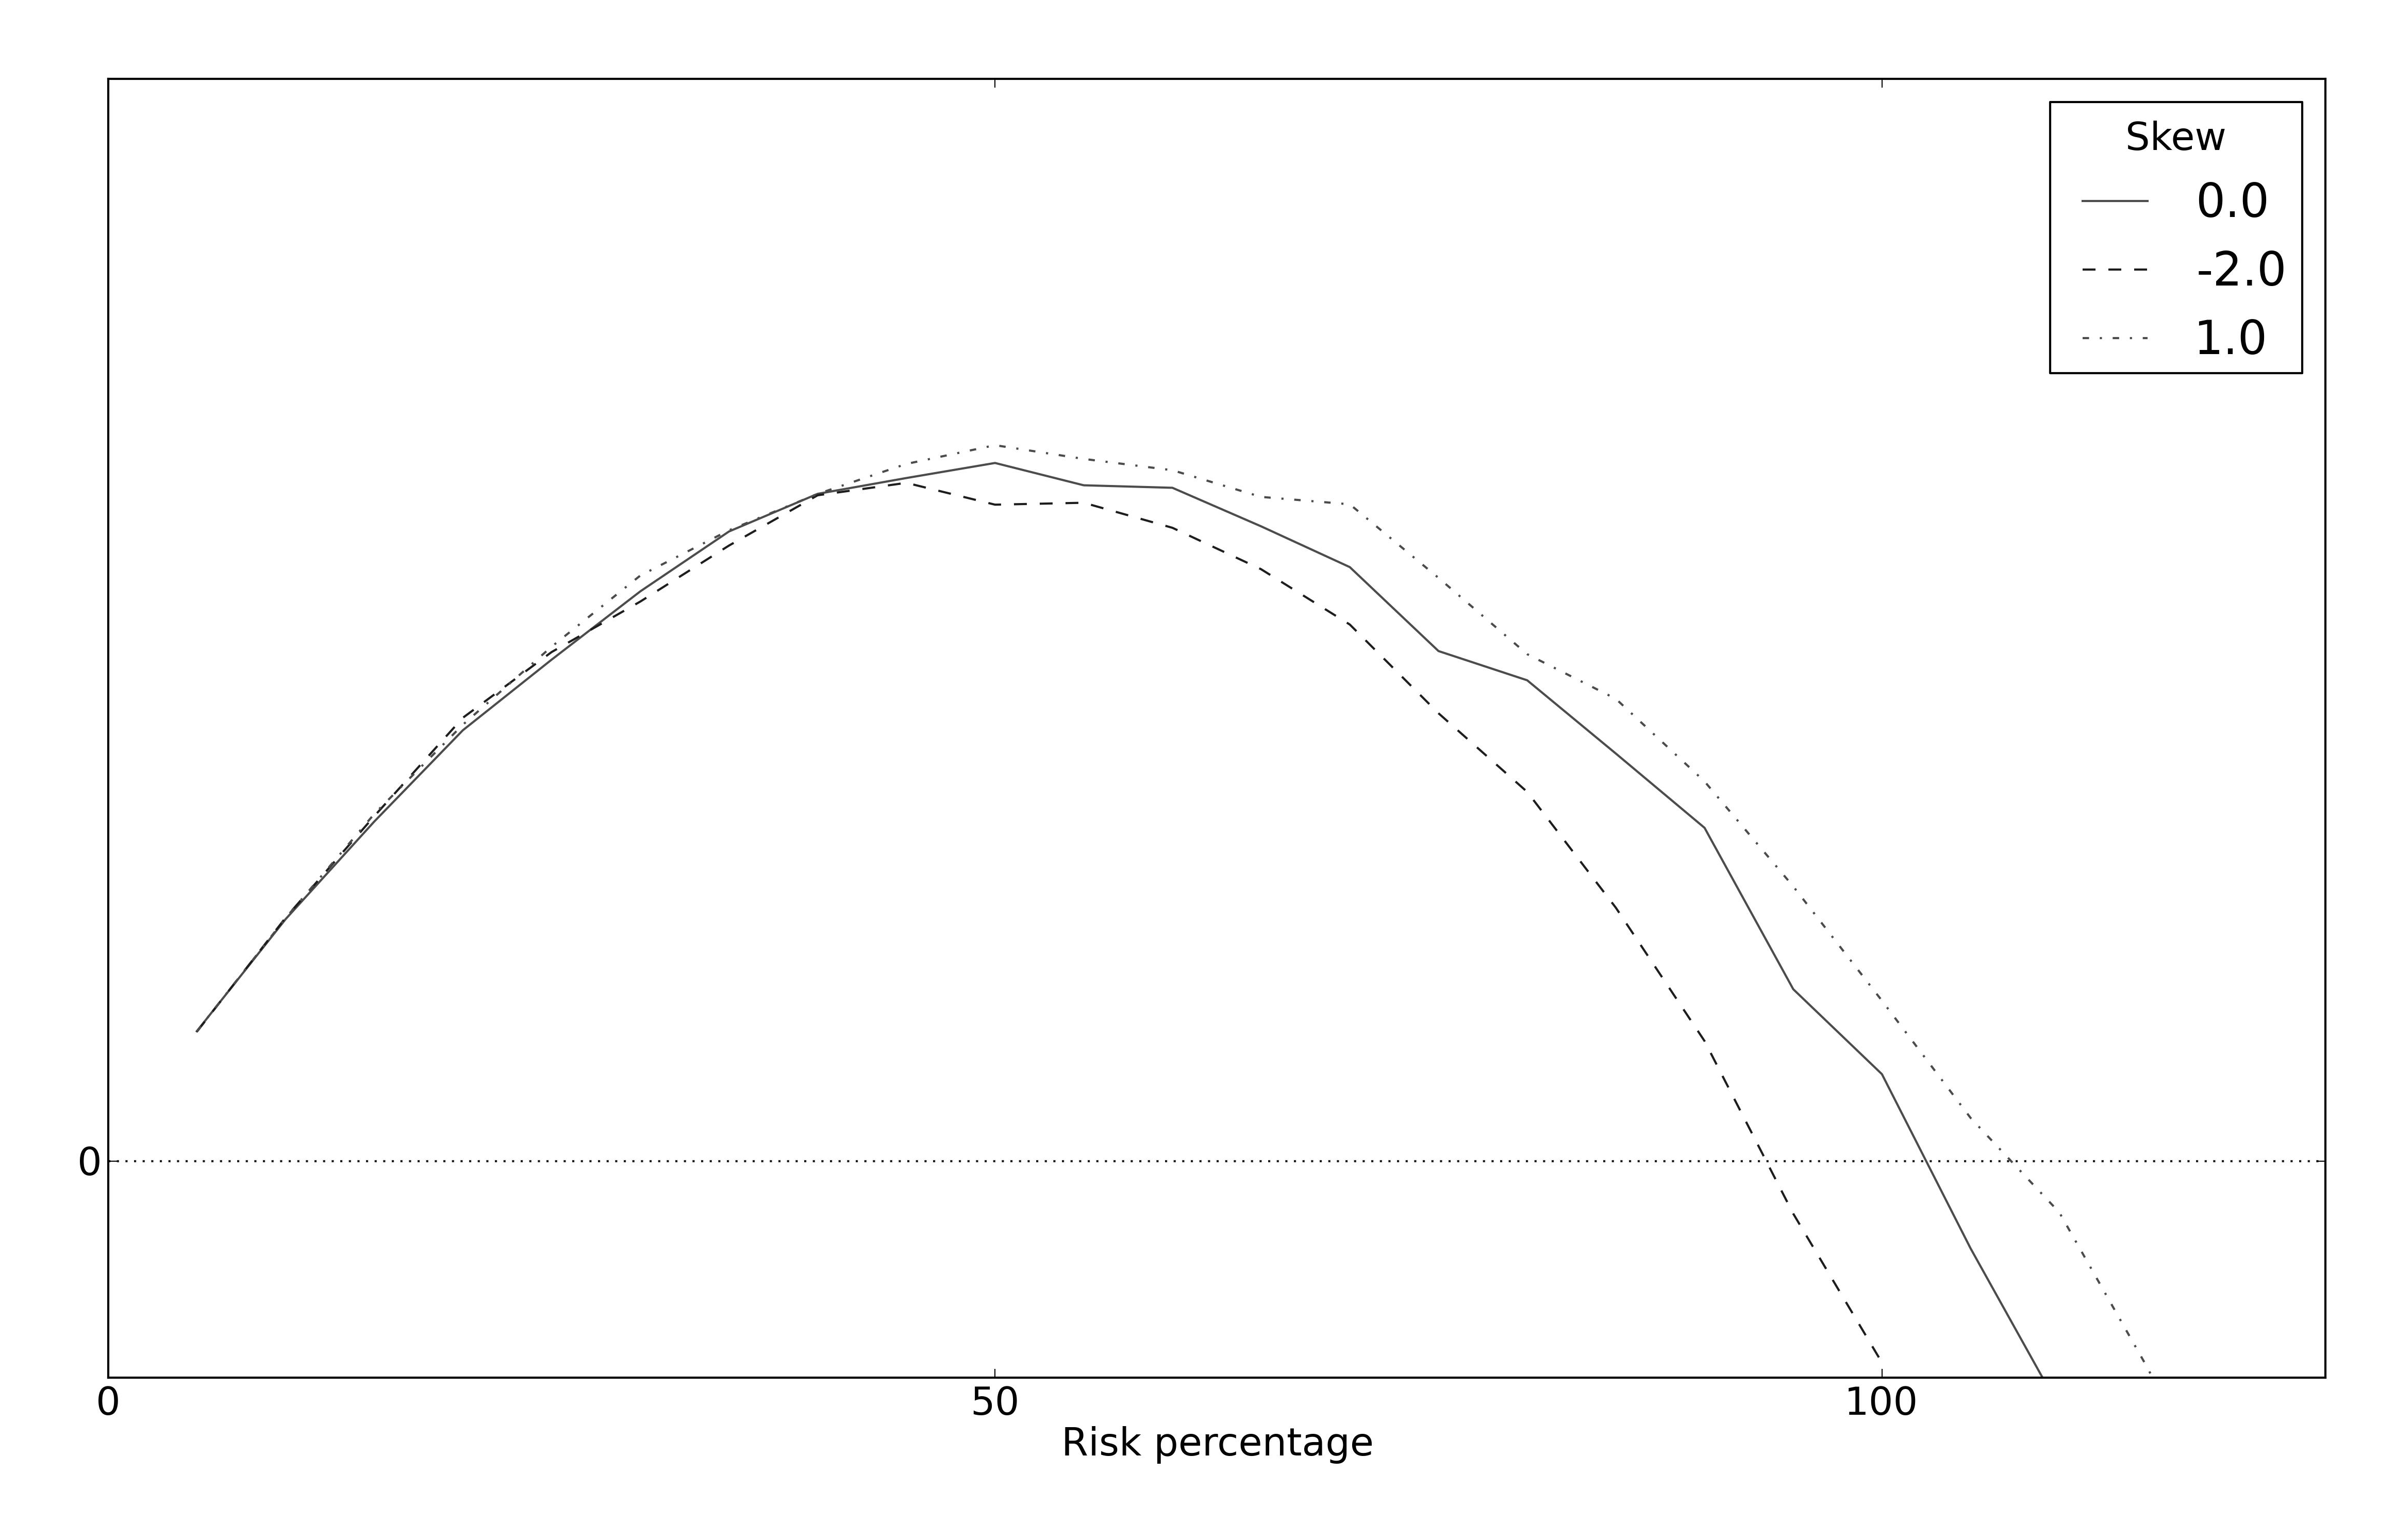
\includegraphics[width=\textwidth]{figures/raw/img-021.png} \caption{KELLY CRITERION IMPLIES THE OPTIMAL RISK PERCENTAGE FOR A SHARPE RATIO 0.5 SYSTEM IS 50\%. WITH HIGHER RISK THINGS GO BADLY, ESPECIALLY FOR NEGATIVE SKEW STRATEGIES.\\
Kelly 准则意味着：对于夏普比率为 0.5 的系统，最优风险百分比是 50\%。如果风险更高，结果就会迅速恶化，尤其是对负偏度策略而言。}\end{figure}

\begin{englishblock} The X-axis shows the percentage volatility target and the Y-axis the geometric mean of returns which Kelly optimises. \end{englishblock}

\begin{chineseblock}横轴表示百分比波动率目标，纵轴表示 Kelly 所优化的收益几何平均值。\end{chineseblock}

\begin{bilingualtableblock} \rawtablecaption{BIG SHARPE MEANS BIGGER RISK AND EXPONENTIALLY BIGGER PROFITS\\更高的夏普意味着更高的风险，也意味着指数级更大的利润}\begingroup \small \centering \begin{tabular}{@{} ccc@{}}
\toprule
\shortstack{Expected\\Sharpe ratio} & \shortstack{Optimum percentage\\volatility target} & \shortstack{Expected\\return} \\
\midrule
0.2 & 20\% & 4\% \\
0.5 & 50\% & 25\% \\
0.5 & 50\% & 25\% \\
0.75 & 75\% & 56\% \\
0.75 & 75\% & 56\% \\
1.0 & 100\% & 100\% \\
1.0 & 100\% & 100\% \\
2.0 & 200\% & 400\% \\
2.0 & 200\% & 400\% \\
\bottomrule
\end{tabular}
\par \endgroup \end{bilingualtableblock}

\begin{englishblock} The table shows the expected annual return (as a percentage of trading capital), given different Sharpe ratio (SR) (rows) and using the optimal Kelly percentage volatility target. Expected return is SR multiplied by percentage volatility target. \end{englishblock}

\begin{chineseblock}这张表展示的是：在不同夏普比率（行）下，使用最优 Kelly 百分比波动率目标时，你能够得到的预期年收益（以交易资本百分比表示）。预期收益等于 SR 乘以百分比波动率目标。\end{chineseblock}

\bipairgap

\begin{englishblock} This finding is potentially dangerous when used by an over confident investor. It's very easy with back-testing software to get over-fitted performance with a Sharpe ratio (SR) of 2, 3 or even higher. If you believe those are attainable then a risk percentage of 100\% or 200\% seems justified. As table 24 shows, running at a 200\% risk with SR of 2.0 implies huge returns of 400\% a year! Unfortunately many people with capital of \$20,000 will conclude it's possible to earn 400\% a year, or \$80,000, as full-time traders. There are also plenty of brokers who will happily provide them with the necessary leverage. Most of these people will quickly lose their \$20,000, as they won't achieve their expected SR. It's very difficult to know exactly what your true Sharpe ratio really would have been in the past, with back-tests giving you only a rough upwardly estimate, and it's utterly impossible to know what SR to expect in the future. Even if you had a crystal ball, and knew your expected Sharpe precisely, you could be unlucky and have a decade or more of sub-par performance. Figure 21 shows that if you realise an SR of only 0.5 then a 200\% volatility target will see you ending up deep underwater. In general if you get your estimate of SR wrong and bet more than the optimal then you have a high chance of losing your shirt. \end{englishblock}

\begin{chineseblock}当一个过度自信的投资者使用这个结论时，它就会变得非常危险。借助回测软件，你很容易就能得到一个过拟合的表现结果，夏普比率（SR）可能高达 2、3，甚至更高。如果你相信这些数字是真实可达的，那么 100\% 甚至 200\% 的风险百分比看起来似乎都合情合理。正如表 24 所示，在 SR 为 2.0 的情况下，以 200\% 风险运行，意味着惊人的 400\% 年收益！不幸的是，很多拥有 \$20,000 资本的人看到这里，就会得出结论：全职交易每年赚 400\%，也就是 \$80,000，是完全可能的。也有很多经纪商会很乐意提供实现这一点所需的杠杆。但这些人中的大多数，很快就会把自己的 \$20,000 亏光，因为他们根本达不到自己预期中的 SR。你其实很难准确知道，自己的真实夏普比率在历史上究竟应该是多少；回测通常只会给你一个偏高的粗略估计，而对于未来到底该期待怎样的 SR，更是根本不可能知道。即便你真的有一颗水晶球，能够精确知道自己的预期夏普，你也仍然可能倒霉，连续十年甚至更久都处在低于预期的表现区间里。图 21 清楚展示了：如果你最后实现的 SR 只有 0.5，那么在 200\% 波动率目标下，你最终会亏得非常惨。一般来说，如果你把 SR 估错了，而且下的注又大于最优水平，那么你有很大概率会把自己输得一干二净。\end{chineseblock}

\bilingualsubsection{Recommended percentage volatility targets}{建议采用的百分比波动率目标}

\begin{englishblock} I run a highly diversified futures trading system with around 45 instruments, eight trading rules drawn from four different styles, and 30 trading rule variations. In a 35 year back-test, conservatively fitted with out of sample bootstrapping, it has a Sharpe ratio (SR) of around 1.0 after costs, but the highest volatility target I'd advocate using \end{englishblock}

\begin{chineseblock}我自己运行的是一套高度分散化的期货交易系统，它包含大约 45 个品种、8 条来自 4 种不同风格的交易规则，以及 30 个交易规则变体。在一项长达 35 年、采用保守的样本外自助法拟合的回测中，它在扣除成本后的夏普比率（SR）大约是 1.0，但我愿意主张使用的最高波动率目标却只有\end{chineseblock}

\bipairgap

\begin{englishblock} for it is 37\%, rather than the 100\% suggested by the Kelly criterion and the back-tested SR.\footnote{At the time of writing I'm using a 25\% volatility target, reflecting my relatively low appetite for risk. \par 在我写这本书的时候，我自己实际采用的是 25\% 的波动率目标，这反映了我个人相对较低的风险偏好。} Why such a conservative number -- am I a wimp? There are several reasons for my caution. Firstly, it's unlikely a back-tested SR will be achieved in the future. On average realised performance is never as good as in back-tests. This is because it's very easy to over-fit if you ignore the advice in chapters three and four. Additionally it's difficult with ideas first testing to avoid using only trading rules that you already know would have worked. Even if you could avoid over-fitting actual profits are unlikely to be as high as they could have been in the past. This is because future asset returns are likely to be lower than in the historical data set we usually use for back-testing, as I discussed in chapter two, ‘Systematic Trading Rules', in the section on achievable Sharpe ratios (from page 46). To find realistic achievable SR from back-test results a good rule of thumb is to use the ratios in table 14 (page 90). These suggest that for an out of sample bootstrap, as I've used in my own system, a ratio of 0.75 should be applied to find a more realistic Sharpe ratio. Much lower ratios should be used if you haven't been as careful with your fitting. I also said in chapter two that I think the absolute maximum SR that staunch systems traders should expect to achieve is 1.0, regardless of how good their back-test is. Secondly, using the full Kelly criteria is far too aggressive, because of the risk of getting a poor run of luck and the large drawdowns that can result, even if SR expectations are correct.\footnote{Here is famous Kelly fan, hedge fund manager and Blackjack card counter Ed Thorpe: "My experience has been that most cautious … investors who use Kelly find the frequency of substantial bankroll reductions to be uncomfortably large." (Quoted in Fortune's Formula.) \par 这里引用一位著名的 Kelly 支持者、对冲基金经理兼二十一点算牌高手 Ed Thorpe 的话：“根据我的经验，大多数谨慎的……使用 Kelly 的投资者，都会觉得资产大幅回撤出现得过于频繁，令人不适。”（引自 \textit{Fortune's Formula}。）} In table 23 someone using the correct Kelly target of 50\% would have a 10\% chance of losing half their money after ten years; which most people would find worrying. It's far better to use Half-Kelly and set your risk at half the optimal. Column A of table 25 shows the recommended percentage volatility target for a given realistic back-tested SR. For my own system I started with the back-tested Sharpe ratio of 1.0. Multiplying by 0.75 (as I'm using out of sample bootstrapping) from table 14, this gives me a realistic SR of 0.75. With full Kelly criterion betting that would be a 75\% volatility target, which I then halved to get 37\% (rounding down). This assumes your trading system, like mine, has zero or positive skew. You should be very careful if you have expected negative skew. As figure 21 shows, the penalty for too much risk is greater with negative skew than when skew is positive, or zero. As I discussed in chapter two, many negative skew strategies have fantastic SR in back-test, but I advise you to run them at half the risk you'd use for a more benign trading system. Column B of table 25 shows the recommended percentage volatility target for negative skew systems. \end{englishblock}

\begin{chineseblock} 37\%，而不是 Kelly 准则和回测 SR 所暗示的 100\%。为什么这个数字如此保守--- 难道我是个胆小鬼吗？我之所以谨慎，有好几个原因。首先，回测得到的 SR 在未来真正实现出来的概率很低。平均而言，真实表现永远不会像回测那样好。原因在于，如果你忽略第三章和第四章中的建议，就会非常容易过拟合。此外，在“先有想法再验证”的测试过程中，你也很难完全避免只去使用那些你本来就知道会有效的交易规则。即便你真的设法避免了过拟合，真实利润也仍然不太可能像过去那样高。这是因为，正如我在第二章“系统化交易规则”关于可实现夏普比率的部分（第 46 页起）所讨论的那样，未来资产收益很可能会低于我们通常用来回测的历史样本。要从回测结果中得到更现实、可实现的 SR，一个不错的经验法则是使用表 14（第 90 页）中的比例。它们表明：如果你像我一样采用样本外自助法，那么应当乘以 0.75，才能得到更现实的夏普比率。如果你在拟合时没有做到这么谨慎，那么还应使用更低的比例。我在第二章中也说过：无论回测结果有多漂亮，我认为坚定的系统化交易者应当期待达到的绝对最大 SR 也不过是 1.0。第二，完整 Kelly 准则实在是太激进了，因为即便你的 SR 预期完全正确，它仍然会让你暴露在坏运气拖累下的巨大回撤风险之中。在表 23 中，一个使用正确 Kelly 目标 50\% 的人，在十年后有 10\% 的概率亏掉一半本金；这对绝大多数人来说都会令人不安。因此，采用半 Kelly，把风险设定为最优值的一半，会好得多。表 25 的 A 列给出了：在某个现实可行的回测 SR 下，我建议采用的百分比波动率目标。以我自己的系统为例，我先从 1.0 的回测夏普比率出发，再根据表 14 乘以 0.75（因为我使用的是样本外自助法），得到更现实的 SR = 0.75。如果按完整 Kelly 准则下注，对应的波动率目标会是 75\%；再把它减半之后，就得到 37\%（向下取整）。这一切都建立在你的交易系统和我的系统一样，偏度为零或正偏度的前提之上。如果你预期系统是负偏度的，就必须格外小心。正如图 21 所展示的那样，风险过高时，负偏度系统所遭受的惩罚会比正偏度或零偏度系统更严重。正如我在第二章中讨论的那样，许多负偏度策略在回测里会有非常漂亮的 SR，但我建议你让这类策略运行在一个更“温和”系统所使用风险的一半水平。表 25 的 B 列，给出了我建议用于负偏度系统的百分比波动率目标。\end{chineseblock}

\begin{bilingualtableblock} \rawtablecaption{WHAT VOLATILITY TARGET SHOULD STAUNCH SYSTEMS TRADERS USE?\\坚定的系统化交易者应使用怎样的波动率目标？}\begingroup \small \centering \begin{tabular}{@{} lcc@{}}
\toprule
Realistic back-tested SR & (A) Skew $>$ 0 & (B) Negative skew \\
现实可行的回测 SR & (A) 偏度 $>$ 0 & (B) 负偏度 \\
\midrule
0.25 & 12\% & 6\% \\
0.25 & 12\% & 6\% \\
0.40 & 20\% & 10\% \\
0.40 & 20\% & 10\% \\
0.50 & 25\% & 12\% \\
0.50 & 25\% & 12\% \\
0.75 & 37\% & 19\% \\
0.75 & 37\% & 19\% \\
1.0 or more & 50\% & 25\% \\
1.0 或以上 & 50\% & 25\% \\
\bottomrule
\end{tabular}
\par \endgroup \end{bilingualtableblock}

\begin{englishblock} The table shows the recommended percentage volatility target for those who can backtest their dynamic trading systems, depending on the skew of returns (columns) and achievable back-tested Sharpe ratios (SR) (rows) after making adjustments to simulated results from table 14 on page 90. Optimal volatility target is calculated using Half-Kelly. For negative skew strategies this is cut in half again. We assume a maximum SR of 1.0 is achievable. \end{englishblock}

\begin{chineseblock}这张表展示的是：对于那些可以回测自己动态交易系统的人来说，在根据第 90 页表 14 对模拟结果进行调整之后，不同收益偏度（列）与可实现的回测夏普比率（行）对应的建议百分比波动率目标。最优波动率目标是用半 Kelly 计算出来的。对于负偏度策略，这个值还要再减半。我们假设可实现的最大 SR 为 1.0。 \end{chineseblock}

\bipairgap

\begin{englishblock} The returns of asset allocating investors are limited by their use of a static trading strategy. With a small, relatively undiversified portfolio you shouldn't expect high Sharpe ratios. As I said in chapter two, if you're holding a dozen equities in different industries but from the same country then you probably will achieve an SR of around 0.20. Those with larger portfolios diversified across multiple asset classes could get a maximum realistic SR of 0.4. Column C of table 26 shows the correct targets given asset allocators' SR expectations. However, as you'll see in chapter fourteen, it's unlikely even this level of volatility can be achieved as these investors don't use leverage. Semi-automatic traders have systems which cannot be back-tested and usually have a small, relatively un-diversified, set of ad-hoc instruments. I would initially assume an achievable SR of 0.20 unless you are very experienced, are trading across multiple asset classes, and have a good track record with real money. As you saw in chapter two, in my opinion an SR of 0.5 is the maximum safe achievable level, so you should set the volatility target at no more than 25\%. Again the target should be halved if you are trading a strategy that is likely to have negative skew, such as selling option volatility, or exhibits a similar return pattern with steady profits on most bets with occasional large losses. Columns D and E of table 26 show the appropriate volatility targets for this type of trader. \end{englishblock}

\begin{chineseblock}资产配置型投资者的收益，会被其静态交易策略本身所限制。对于一个规模较小、分散化程度也不高的投资组合来说，你不应期待它拥有很高的夏普比率。正如我在第二章中说过的，如果你持有十几只来自同一国家、但分属不同行业的股票，那么你大概只能实现 0.20 左右的 SR。而那些在多个资产类别之间进行分散化、且投资组合规模更大的投资者，能够获得的现实最大 SR 大约是 0.4。表 26 的 C 列，展示了在资产配置型投资者 SR 预期下应当采用的正确目标。不过，正如你会在第十四章中看到的，由于这些投资者不使用杠杆，他们甚至未必能够实现这个水平的波动率。半自动交易者所使用的系统无法回测，而且通常只会持有一组规模较小、分散度也不高的临时性品种。除非你经验非常丰富、横跨多个资产类别交易，并且有不错的真钱交易记录，否则我一开始会假设可实现 SR 只有 0.20。正如你在第二章中看到的那样，在我看来，0.5 的 SR 已经是一个安全意义上的可实现上限，因此你的波动率目标不应高于 25\%。同样地，如果你交易的是一套很可能带有负偏度的策略，比如卖出期权波动率，或者其收益模式与此类似--- 大多数时候稳定赚钱，但偶尔会遭遇巨大亏损--- 那么这个目标还应再减半。表 26 的 D 列和 E 列，就给出了这类交易者应当采用的合适波动率目标。\end{chineseblock}

\begin{bilingualtableblock} \rawtablecaption{WHAT VOLATILITY TARGET SHOULD ASSET ALLOCATING INVESTORS AND SEMI- AUTOMATIC TRADERS USE?\\资产配置型投资者与半自动交易者应使用怎样的波动率目标？}\begingroup \small \centering
\resizebox{\textwidth}{!}{%
\begin{tabular}{@{} lccc@{}}
\toprule
Expected SR & (C) Asset allocating investor & (D) Semi-automatic trader, zero or positive skew & (E) Semi-automatic trader, negative skew \\
预期 SR & (C) 资产配置型投资者 & (D) 半自动交易者，零偏度或正偏度 & (E) 半自动交易者，负偏度 \\
\midrule
0.20 & 10\% & 10\% & 5\% \\
0.20 & 10\% & 10\% & 5\% \\
0.30 & 15\% & 15\% & 7\% \\
0.30 & 15\% & 15\% & 7\% \\
0.40 & 20\% & 20\% & 10\% \\
0.40 & 20\% & 20\% & 10\% \\
0.5 or more & 20\% & 25\% & 12\% \\
0.5 或以上 & 20\% & 25\% & 12\% \\
\bottomrule
\end{tabular}%
}
\par \endgroup \end{bilingualtableblock}

\begin{englishblock} This table shows the recommended percentage volatility target depending on the type of trader and expected skew (columns), and Sharpe ratio (SR) expectations (rows). The optimal volatility target is calculated using Half-Kelly. We assume asset allocators shouldn’t expect more than 0.40 SR and semi-automatic traders won’t get more than 0.50 SR. Asset allocators are assumed to have zero skew. We halve volatility targets for negative skew semi-automatic trading. \end{englishblock}

\begin{chineseblock}这张表展示的是：根据交易者类型与预期偏度（列），以及夏普比率（SR）预期（行），所对应的建议百分比波动率目标。最优波动率目标采用半 Kelly 计算。我们假设资产配置型投资者不应期待超过 0.40 的 SR，而半自动交易者不应期待超过 0.50 的 SR。资产配置型投资者被假定为零偏度。对于负偏度的半自动交易策略，我们再把波动率目标减半。\end{chineseblock}

\bipairgap

\begin{englishblock}
This implies that nobody will use more than a maximum 50% volatility target and most
people should use less. Tables 20 to 23 illustrate that a 50% annualised volatility will
mean some pretty substantial losses from time to time. Just because the volatility targets in tables 25 and 26 are optimal it doesn’t mean they will suit you, or that your broker will permit them. It just means you should never run a higher risk target than this. \end{englishblock}

\begin{chineseblock}这意味着，没有人应当使用超过 50\% 的最大波动率目标，而大多数人都应当使用更低的值。表 20 到表 23 已经说明，50\% 的年化波动率意味着你会不时遭遇相当可观的亏损。表 25 和表 26 中给出的波动率目标即便是“最优”的，也不代表它们就一定适合你，更不代表你的经纪商会允许你这么做。它们真正表达的只是：你永远不应该把风险目标设得比这个更高。\end{chineseblock}

\bilingualsubsection{When the percentage volatility target should be changed}{什么时候应该调整百分比波动率目标}

\begin{englishblock} I don’t advocate changing your percentage volatility target since there is a potential risk of meddling; reducing it when you don’t trust your system and increasing it when it agrees with you. The exception is if you have grossly miscalculated your tolerance for risk. You begin trading on day one with a 50\% target, but the first big loss then sends you or your investors into a panic. In this case you should significantly reduce your percentage target. However it should ideally be a one off change and only ever downwards. To avoid this scenario it’s better to start with significantly lower trading capital and gradually increase it until you have the full amount invested. Keep the percentage volatility target fixed and allow your cash volatility to increase up to the point just before you get uncomfortable. This also helps with gaining confidence in your trading strategy and testing any automated systems. \end{englishblock}

\begin{chineseblock}我并不主张频繁改变你的百分比波动率目标，因为这样存在干预风险：当你不信任系统时就把目标调低，而当系统恰好与你想法一致时就把目标调高。唯一的例外，是你显著地误判了自己对风险的承受能力。比如你在第一天就带着 50\% 的目标开始交易，可第一笔大亏就让你或你的投资者陷入了恐慌。在这种情况下，你就应当显著降低自己的百分比目标。但理想情况下，这应当是一次性的调整，而且只会是向下调整。为了避免这种局面，更好的方法是：从显著更低的交易资本开始，然后逐渐把资金加到最终你真正想投入的规模。保持百分比波动率目标固定不变，让现金波动率随着资本增长逐步升高，直到接近、但还没有超出你的舒适边界。这同时也有助于你建立对交易策略的信心，并测试任何自动化系统。\end{chineseblock}

\bilingualsection{Rolling up profits and losses}{把盈亏滚动进资本}

\begin{englishblock} Once set your percentage volatility target shouldn't need changing. However your trading capital will definitely change from its initial value. This implies that your cash volatility target will also be adjusted over time. Let's imagine you have trading capital of \$100,000\footnote{I've assumed a Sharpe ratio (SR) of 0.5 here, and the returns are drawn from a Gaussian normal distribution. Using a different SR won't affect these numbers much, although the annual loss figures will be slightly better (worse) if the true Sharpe is higher (lower). \par 这里我假设夏普比率（SR）为 0.5，且收益服从高斯正态分布。若使用不同的 SR，这些数值变化不会太大，尽管若真实夏普更高（更低），年度亏损数字会略微更好（更差）。} and after reading this chapter you've decided on a 30\% volatility target. You begin trading with the appropriate \$30,000 annualised cash volatility target. Then on day one you lose \$2,000. Should you continue to use a \$30,000 volatility target? You should not. The implication of the Kelly criterion is that you should adjust your risk according to your current capital. You did have \$100,000 of capital, but now you only have \$98,000. Instead of having a 30\% volatility target (\$30,000 of \$100,000) you effectively have a target of \$30,000 divided by \$98,000 = 30.6\%. This might not seem a big deal, but you are now betting more than you intended and you've slightly increased your chances of going bankrupt. If you make further losses the situation could deteriorate fast. The correct thing to do is to reduce your volatility target to 30\% of your current capital of \$98,000, or \$29,400. Now suppose things start to improve and you make \$2,000 back. Your accumulated losses have reduced to zero and your volatility target will be back to 30\% of \$100,000, or \$30,000. After another profitable day making \$3,000 you're now in positive territory with an account value of \$103,000\footnote{The results would be slightly worse for negative skew, and slightly better for positive skew. For example with a 200\% volatility target the chances of losing half your capital over ten years are 90\% with positive skew of 1.0 and 97\% with negative skew of -2.0. \par 若是负偏度，结果会略差；若是正偏度，结果会略好。比如在 200\% 的波动率目标下，十年内亏掉一半资金的概率，在偏度为 1.0 时是 90\%，而在偏度为 -2.0 时则是 97\%。} -- higher than your starting capital. Should you now increase your risk appetite above its initial level? If you want to maximise your wealth then Kelly says you should roll up your profits and increase your capital.\footnote{Someone who is trading as a hobby and starting with a small stake would probably do this. Those investing other people's money should also add all profits after fees to their trading capital, so that returns are compounded, unless they are committed to paying coupons or guaranteeing a certain proportion of the initial investment made. If you are more risk averse then rolling up profits might not make sense, if for example you live partly or wholly off your trading income. This is the approach that I take. \par 如果有人只是把交易当作爱好，并且起始资金很小，那么他大概率会这么做。那些管理他人资金的人，也应当把扣除费用后的全部利润重新计入交易资本，让收益滚动复利，除非他们承诺要持续支付利息，或对初始投资中的某个比例作出保本保证。如果你更厌恶风险，那么把利润全部滚回去可能就不一定合理；例如，如果你部分或完全依赖交易收入来生活。这也是我自己所采取的做法。} The new volatility target will be 30\% of \$103,000, or \$30,900. This means you will be compounding your returns, which over the long run will increase them faster. You should also reduce your trading capital, and hence your cash volatility target, if you withdraw money from your trading account or investors redeem. Similarly if you put more funds in then you would normally increase your maximum capital. There are exceptions such as if you are putting cash into a leveraged account to meet margin or reduce borrowing, but you don't want to increase the amount of capital at risk. In my own trading an automated process checks my account value, and adjusts risk accordingly, on an hourly basis. If your system is not automated and if you are running with more than a 15\% volatility target I would recommend checking at least daily. With a lower target you can check more infrequently, but if you're using leverage I'd advise always calculating your volatility target at least once a week. \end{englishblock}

\begin{chineseblock}一旦设定好，你的百分比波动率目标原则上就不需要再变了。然而，你的交易资本本身肯定会偏离初始值。这就意味着，你的现金波动率目标也应当随着时间不断调整。假设你有 \$100,000 的交易资本，并且读完本章后决定采用 30\% 的波动率目标。那么你一开始交易时，对应的年化现金波动率目标就是 \$30,000。接着，第一天你亏了 \$2,000。你还应该继续使用 \$30,000 的波动率目标吗？答案是不应该。Kelly 准则的含义之一，就是你应当根据当前资本来调整风险。你原本有 \$100,000 的资本，但现在只剩下 \$98,000。如果你仍继续使用 \$30,000 的现金波动率目标，那么相当于你现在实际上承担的是 \$30,000 ÷ \$98,000 = 30.6\% 的风险目标。这看起来也许差距不大，但你实际上已经下注得比原本打算更多了一点，也略微提高了自己破产的概率。如果你继续亏损，情况就可能迅速恶化。正确做法，是把波动率目标降到当前资本 \$98,000 的 30\%，也就是 \$29,400。现在假设事情开始好转，你又赚回了 \$2,000。此时你的累计亏损归零，而你的波动率目标也会回到 \$100,000 的 30\%，即 \$30,000。又过了一天，你再赚 \$3,000，那么你现在账户值就是 \$103,000，已经高于初始资本。此时你是否应该把风险偏好抬到高于最初水平？如果你的目标是最大化财富，那么 Kelly 会告诉你：你应当把利润滚入资本，随之增加风险资本。新的波动率目标就会是 \$103,000 的 30\%，也就是 \$30,900。这意味着你会开始对收益进行复利滚动，而长期来看，这会让你的财富增长更快。如果你从交易账户中提取了资金，或者投资者进行了赎回，你也应当相应减少交易资本，进而降低现金波动率目标。反过来，如果你追加了新资金，那么通常也应当相应提高最大资本规模。当然也有例外，比如你向杠杆账户中补充现金只是为了满足保证金要求，或者为了减少借款，但你并不想增加实际在风险中的资本规模。就我自己的交易而言，我有一套自动化流程，每小时检查一次账户价值，并据此调整风险。如果你的系统还没有自动化，而且你运行的波动率目标高于 15\%，那么我建议至少每天检查一次。如果目标更低，你可以降低检查频率；但如果你在使用杠杆，那我建议你至少每周计算一次波动率目标。\end{chineseblock}

\bilingualsection{What percentage of capital per trade?}{每笔交易占资本的百分比是多少？}

\begin{englishblock} Traditional money management systems allocate a certain percentage of trading capital to be risked on each trade or bet. If you're familiar with these systems you might be wondering how this relates to the volatility targeting done here. It is possible to infer the percentage volatility target that is implied for a particular trading system if you know the approximate holding period, the average number of positions held and the maximum amount of capital put at risk on each trade. You just need to assume that the average bet is half the maximum, which is the same ratio between my recommended average forecast of 10 and maximum of 20. Table 27 gives the results, assuming an average of two positions are held at once. If a greater or fewer number are traded on average, then you just need to multiply or divide the figures appropriately. So with an average of four positions you'd double them, and for a single position halve them. \end{englishblock}

\begin{chineseblock}传统的资金管理系统，通常会规定：每笔交易或下注只允许承担交易资本的一定百分比风险。如果你熟悉这类系统，你也许会想知道，它与这里所做的波动率目标设定到底是什么关系。如果你知道某套交易系统的大致持仓周期、平均持仓数量，以及每笔交易所承担的最大资本风险，那么其实可以反推出它所隐含的百分比波动率目标。你只需要再加一个假设：平均下注规模等于最大下注规模的一半，这正好对应我所建议的平均预测值 10 与最大预测值 20 之间的比例关系。表 27 给出了在平均同时持有两笔头寸时的结果。如果你平均持有的头寸更多或更少，那你只需要相应地乘上或除以合适的比例即可。例如，如果平均持有四个头寸，就把表中的数字乘以 2；如果只有一个头寸，就把它们除以 2。 \end{chineseblock}

\begin{bilingualtableblock} \rawtablecaption{WHAT IS THE VOLATILITY IMPLIED BY A TRADING SYSTEM'S HOLDING PERIOD AND BET SIZE?\\一个交易系统的持仓周期与下注规模，隐含了怎样的波动率？}\begingroup \small \centering
\resizebox{\textwidth}{!}{%
\begin{tabular}{@{} lccccc@{}}
\toprule
& \multicolumn{5}{c}{Maximum percentage of capital at risk per trade} \\
& \multicolumn{5}{c}{每笔交易可承担的最大资本风险百分比} \\
\cmidrule(l){2-6}
Average holding period & 1\% & 2.5\% & 5\% & 10\% & 20\% \\
平均持仓周期 & 1\% & 2.5\% & 5\% & 10\% & 20\% \\
\midrule
1 day & 40\% & 100\% & 200\% & ! & ! \\
1 天 & 40\% & 100\% & 200\% & ! & ! \\
1 week & 16\% & 40\% & 80\% & 160\% & ! \\
1 周 & 16\% & 40\% & 80\% & 160\% & ! \\
2 weeks & 8\% & 19\% & 38\% & 76\% & 152\% \\
2 周 & 8\% & 19\% & 38\% & 76\% & 152\% \\
6 weeks & 4\% & 10\% & 21\% & 41\% & 82\% \\
6 周 & 4\% & 10\% & 21\% & 41\% & 82\% \\
3 months & 3\% & 7\% & 13\% & 27\% & 53\% \\
3 个月 & 3\% & 7\% & 13\% & 27\% & 53\% \\
\bottomrule
\end{tabular}%
}
\par \endgroup \end{bilingualtableblock}

\begin{englishblock} The table shows the implied annualised percentage volatility target for a given average holding period (rows) and maximum percentage of capital allocated to each bet (columns), assuming an average of two bets are held in the portfolio. "!" indicates volatility greater than 200\% per year. \end{englishblock}

\begin{chineseblock}这张表展示的是：在假设平均同时持有两笔下注的情况下，不同平均持仓周期（行）以及每笔下注所承担的最大资本比例（列）所隐含的年化百分比波动率目标。“!” 表示波动率高于每年 200\%。 \end{chineseblock}

\bipairgap

\begin{englishblock} As an example take the system which I briefly discussed in the introductory chapter. This held positions for around a week, with no more than 10\% of capital at risk. Let's assume on average that two bets are made at once, although the author wasn't clear on this point (a common shortcoming in trading books). \end{englishblock}

\begin{chineseblock}举个例子，我们来看我在导言章节中曾经简要提到过的那套系统。它平均持仓大约一周，每笔交易承担的资本风险不超过 10\%。我们再假设，平均同时持有两笔下注，尽管原作者对此并没有说清楚（这是交易书里一个很常见的缺陷）。\end{chineseblock}

\bipairgap

\begin{englishblock} This all sounds fairly sedate but from the table this works out to a suicidal 160\% volatility target. If this target is Kelly optimal then the achievable Sharpe ratio must be at least 1.6, implying an expected return of 1.6 × 160\% or 256\% a year! There is some serious overconfidence at work here. Worse still, this is nowhere near the most aggressive system I've ever seen. \end{englishblock}

\begin{chineseblock}听上去这一切似乎还算平稳，但根据表中的换算，它其实对应的是一个接近自杀式的 160\% 波动率目标。如果这个目标真的是 Kelly 意义上的最优，那么可实现的夏普比率至少得有 1.6，这就意味着预期收益将达到 1.6 × 160\%，也就是每年 256\%！这里面显然存在着非常严重的过度自信。更糟的是，这甚至还远远不是我见过最激进的系统。\end{chineseblock}

\bilingualsection{Summary of volatility targeting}{波动率目标设定总结}

\begin{englishblock} Percentage Desired long run expectation of annualised standard deviation of volatility target percentage portfolio returns. A maximum of: • The level of risk that you are comfortable with given tables 20 to 23. • What is practically attainable given your access to leverage and the natural risk of your instruments (see the asset allocating investor example in part four for more details). • The highest level that is safe given the natural volatility of your instruments, and how much leverage they need. Avoid very low volatility instruments requiring insanely high leverage. • The recommended percentage volatility in tables 25 and 26, depending on the back-tested or expected Sharpe ratio and skew of your trading system, and the type of trader or investor you are. Percentage volatility target should remain unchanged. \end{englishblock}

\begin{chineseblock}百分比波动率目标 这是你对投资组合年化收益标准差的长期预期。它的最大值应受以下几项限制：• 根据表 20 到表 23，你自己能够接受的风险水平。• 考虑到你能获得多少杠杆，以及你的工具本身具有怎样的天然风险，从现实角度究竟能达到怎样的水平（更多细节见第四部分中资产配置型投资者的示例）。• 在考虑品种天然波动率和所需杠杆之后，依然安全可行的最高风险水平。应当避开那些天然波动率极低、却需要疯狂高杠杆的工具。• 根据你的交易系统回测或预期的夏普比率与偏度，以及你属于哪一类交易者或投资者，在表 25 与表 26 中所建议的百分比波动率。百分比波动率目标本身应当保持不变。\end{chineseblock}

\bipairgap

\begin{englishblock} Trading capital The amount of capital you currently have at risk in your account. Every day you should add profits and any injections of funds. Deduct any losses and withdrawals made from the account. Measured in currency. \end{englishblock}

\begin{chineseblock}交易资本 这是你账户中当前真正处于风险之中的资本规模。每天都应把盈利和新增资金计入，把亏损和提款扣除。它用货币金额来衡量。\end{chineseblock}

\bipairgap

\begin{englishblock} Annualised Long run expectation of annualised standard deviation of daily portfolio cash volatility returns. Equal to the trading capital multiplied by the percentage volatility target target. Measured in currency. \end{englishblock}

\begin{chineseblock}年化现金波动率目标 这是投资组合日收益标准差的长期年化预期。它等于交易资本乘以百分比波动率目标，用货币金额衡量。\end{chineseblock}

\bipairgap

\begin{englishblock} Daily cash Long run expectation of daily standard deviation of daily portfolio returns. volatility target Annualised cash volatility target divided by ‘the square root of time', which for a 256 business day year is 16. Measured in currency. \end{englishblock}

\begin{chineseblock}日现金波动率目标 这是投资组合日收益标准差的长期预期。它等于年化现金波动率目标除以“时间平方根”；对于一年 256 个交易日而言，这个除数就是 16。它同样以货币金额衡量。\end{chineseblock}

\bipairgap

\begin{englishblock} In the next chapter I will come back to the final piece of advice I got from Sergei and think about how the risk of an instrument determines what size position we should take. \end{englishblock}

\begin{chineseblock}下一章中，我会回到 Sergei 给我的最后一条建议，讨论某个品种本身的风险，究竟是如何决定我们应该持有多大仓位的。\end{chineseblock}
